\section{Gestión de la información}

  \paragraph{}Para todas y cada una de las zonas de las que se compone esta
  aplicación (Administrador principal, Administrador de centro, Asesor y
  Alumno), la interfaz compartirá bastantes detalles en común, diferenciándose
  cada una de ellas del resto en el contenido que puede ver y gestionar el
  usuario que está ejecutando la aplicación, teniendo en cuenta el rol con el
  que participa. Por ejemplo, un usuario asesor no podrá ver determinadas zonas
  para la creación de una nueva titulación, ya que es una tarea que no le
  concierne.

  \paragraph{}Teniendo en cuenta lo anterior, a continuación se muestra una
  captura de pantalla para ejemplificar el diseño de la interfaz común a todas
  las zonas de la aplicación. Se ha utilizado la zona del Administrador
  principal por ser la más completa; pero, como se ha comentado antes, el resto
  de zonas comparten los mismos criterios de diseño, por lo cual la
  navegabilidad y usabilidad no varía entre zonas. La figura
  \ref{capturaGestionInformacion} muestra un ejemplo del diseño de la interfaz
  común.

  \begin{figure}[!ht]
    \begin{center}
      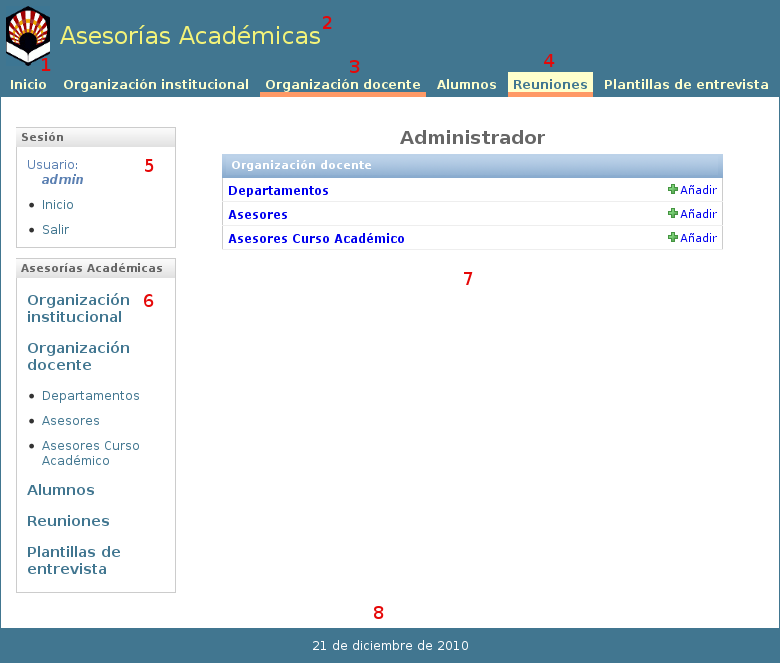
\includegraphics[scale=0.6]{3.Caracteristicas_Interfaz/3.3.Gestion_Informacion/gestion_informacion.png}
      \caption{Captura de pantalla de la gestión de la información.}
      \label{capturaGestionInformacion}
    \end{center}
  \end{figure}


  \paragraph{}Los elementos de la interfaz a destacar están señalados en la
  imagen con números. A continuación se pasan a detallar:

  \begin{enumerate}
    \item \textbf{Logotipo de la Universidad de Córdoba}. Se trata de un
    enlace que, al pinchar sobre él, nos lleva directamente a la página
    principal de la Universidad de Córdoba (\url{http://www.uco.es}).
    \item \textbf{Nombre completo de la aplicación}.
    \item \textbf{Sección activa}. Se trata de la sección de la aplicación donde
    se encuentra el usuario en un momento determinado.
    \item \textbf{Ir a sección}. Se activa cuando el cursor del ratón se
    encuentra encima del enlace a una determinada sección. Si pulsamos el botón
    del ratón, navegaremos hasta la sección indicada.
    \item \textbf{Menú de sesión}. Este menú contiene detalles acerca de la
    sesión que se encuentra ejecutando en un momento determinado.
    \begin{itemize}
      \item Para todas las zonas de la aplicación (Administrador principal,
      Administrador de centro, Asesor y Alumno), estará visible el nombre de
      usuario que ha iniciado la sesión, así como un enlace directo para ir al
      inicio de cada zona, y un enlace para salir de la sesión, el cual
      desconecta al usuario del sistema.
      \item Para la zona del administrador de centro, se mostrará, además,
      el centro que sea objeto de administración en ese momento.
      \item Para las zonas de Asesor y Alumno, se mostrará, además, el curso
      académico que sea objeto de administración en ese momento.
    \end{itemize}

    \item \textbf{Menú de secciones}. Es un menú de accesos rápidos para las
    distintas opciones de las que se compone la sección en la que se encuentra
    el usuario en un determinado momento, así como accesos al resto de
    secciones de la aplicación.
    \item \textbf{Contenido}. En la zona de contenido se mostrará la distinta
    información que sea necesario detallar en cada momento, teniendo en cuenta
    dónde se encuentre el usuario en un determinado momento.
    \item \textbf{Pie de página}. Zona utilizada para exponer alguna otra
    información que se quiera reflejar. Para esta aplicación se ha utilizado
    la fecha actual como información en el pie de página.
  \end{enumerate}

  \subsection{Lista de elementos}

  \paragraph{}La figura \ref{capturaListaElementos} muestra un ejemplo de
  listado de elementos. Como se puede observar, además aparecen elementos
  importantes que es necesario comentar:

  \begin{itemize}
   \item \textbf{Crear nuevos elementos}. Si el usuario dispone de los permisos
   necesarios aparecerá un icono, representado por una cruz verde junto con el
   texto \textit{Añadir nuevo}, que permitirá la adición de nuevos elementos.
   \item \textbf{Generar PDF}. Exporta el listado actual al formato PDF.
   \item \textbf{Búsqueda}. Se permite realizar búsquedas entre los elementos
   que componen la lista mostrada. La figura \ref{capturaBusquedaElementos}
   muestra un ejemplo de búsqueda de elementos.
   \begin{figure}[!ht]
    \begin{center}
      \fbox{
        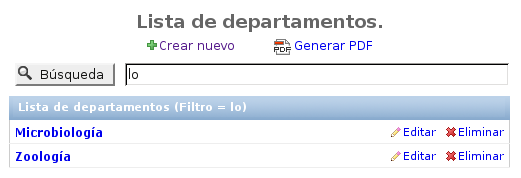
\includegraphics[scale=0.6]{12.Disenyo_Interfaz/12.3.Gestion_Informacion/12.3.1.Lista_Elementos/busqueda_elementos.png}
      }
      \caption{Captura de pantalla de una búsqueda de elementos.}
      \label{capturaBusquedaElementos}
    \end{center}
  \end{figure}
   \item \textbf{Ordenamiento}. Como cabecera de la lista de elementos,
   aparecerá el nombre del conjunto de elementos junto con una flecha indicando
   el tipo de ordenamiento: ascendente o descendente. Si se trata de elementos
   de tipo cadena su ordenamiento se realizará por orden alfabético, y si se
   trata de elementos numéricos de mayor a menor y viceversa.
   \item \textbf{Editar elemento}. Si el usuario dispone de los permisos
   necesarios aparecerá un icono, representado por un lápiz junto con el texto
   \textit{Editar}, que permitirá editar el elemento indicado.
   \item \textbf{Eliminar elemento}. Si el usuario dispone de los permisos
   necesarios aparecerá un icono, representado por una cruz roja girada 45
   grados con respecto a la vertical junto con el texto \textit{Eliminar}, que
   permitirá eliminar el elemento indicado, previa confirmación.
  \end{itemize}

  \begin{figure}[!ht]
    \begin{center}
      \fbox{
        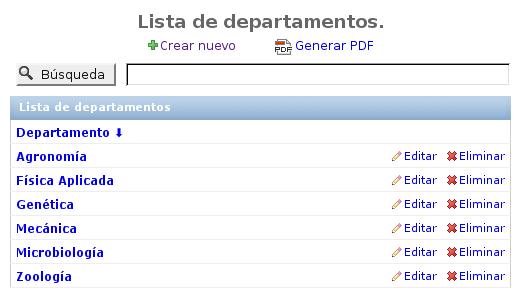
\includegraphics[scale=0.6]{12.Disenyo_Interfaz/12.3.Gestion_Informacion/12.3.1.Lista_Elementos/lista_elementos.png}
      }
      \caption{Captura de pantalla de un listado de elementos.}
      \label{capturaListaElementos}
    \end{center}
  \end{figure}
  \subsection{Adición de elementos}

  \paragraph{}La figura \ref{capturaAdicionElementos} muestra un ejemplo de
  creación de un nuevo elemento. Se puede observar que los campos que dependen
  de otras entidades vienen representados por una lista desplegable, donde se
  debe elegir el elemento al que hacer referencia. El resto de campos se
  introducirán a través de cajas de texto. Por último aparece un botón
  denominado \textit{Confirmar}, el cual intentará crear el elemento en el
  sistema.

  \begin{figure}[!ht]
    \begin{center}
      \fbox{
        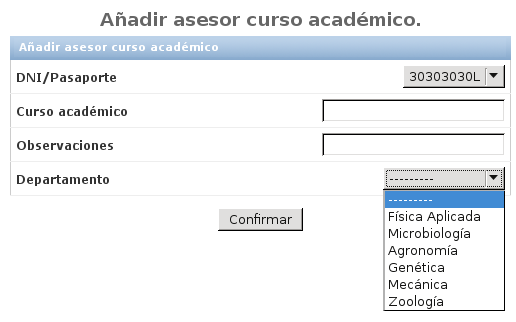
\includegraphics[scale=0.6]{3.Caracteristicas_Interfaz/3.3.Gestion_Informacion/3.3.2.Adicion_Elementos/adicion_elementos.png}
      }
      \caption{Captura de pantalla de la creación de un nuevo elemento.}
      \label{capturaAdicionElementos}
    \end{center}
  \end{figure}

  \item Prueba de actualización de elementos.
  \begin{itemize}
    \item \textbf{Descripción:} Comprobación de actualización de elementos
    en el sistema por los usuarios autorizados. Se ha comprobado la
    actualización de los siguientes elementos para los usuarios indicados a
    continuación:

    \begin{itemize}
      \item Administrador principal.
      \begin{itemize}
        \item Centro.
        \item Administrador de centro.
        \item Centro - Administrador de centro.
        \item Titulación.
        \item Asignatura.
        \item Asignatura Curso Académico.
        \item Departamento.
        \item Asesor.
        \item Asesor Curso Académico.
        \item Alumno.
        \item Alumno Curso Académico.
        \item Matrícula.
        \item Calificación Convocatoria.
        \item Reunión.
        \item Reunión - Pregunta de asesor.
        \item Reunión - Pregunta oficial.
        \item Plantilla de entrevista oficial.
        \item Pregunta oficial.
        \item Plantilla de entrevista de asesor.
        \item Pregunta de asesor.
      \end{itemize}
      \item Administrador de centro.
      \begin{itemize}
        \item Contraseña.
        \item Titulación.
        \item Asignatura.
        \item Matrícula.
        \item Calificación Convocatoria.
      \end{itemize}
      \item Asesor.
      \begin{itemize}
        \item Plantilla de asesor.
        \item Pregunta de asesor.
        \item Reunión individual.
        \item Reunión grupal.
        \item Información personal
        \item Contraseña.
        \item Pregunta de reunión.
      \end{itemize}
      \item Alumno
      \begin{itemize}
        \item Información personal.
        \item Contraseña.
        \item Pregunta de reunión.
      \end{itemize}
    \end{itemize}

    \item \textbf{Problemas encontrados:} No se han encontrado problemas
    funcionales en la actualización de elementos.
    \item \textbf{Soluciones adoptadas:} -
  \end{itemize}

  \subsection{Eliminación de elementos}

  \paragraph{}Para eliminar un elemento del sistema,  es necesario pulsar el
  icono \textit{Eliminar}. Se puede ver una captura de pantalla de este
  icono en la figura \ref{capturaDelElemento}.

  \begin{figure}[!ht]
    \begin{center}
      \fbox{
      
\includegraphics[scale=0.6]{12.Disenyo_Interfaz/12.3.Gestion_Informacion/12.3.4.Eliminacion_Elementos/delElemento.png}
      }
      \caption{Captura de pantalla del icono \textit{Eliminar}.}
      \label{capturaDelElemento}
    \end{center}
  \end{figure}

  \paragraph{}Al pulsar en el icono, se enlazará con la ventana de confirmación
  para eliminar el elemento. Esta ventana se puede ver en la imagen
  \ref{capturaConfirmacion}.

  \begin{figure}[!ht]
    \begin{center}
      \fbox{
      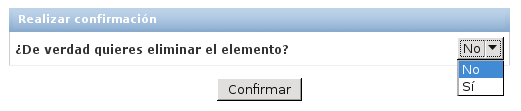
\includegraphics[scale=0.6]{12.Disenyo_Interfaz/12.3.Gestion_Informacion/12.3.4.Eliminacion_Elementos/pantalla_confirmacion.png}
      }
      \caption{Captura de pantalla de la ventana de confirmación para \textit{Eliminar} un elemento.}
      \label{capturaConfirmacion}
    \end{center}
  \end{figure}

  \paragraph{}Una vez realizada la confirmación, se pulsará el botón
  \textit{Confirmar}, el cual se puede ver en la figura
  \ref{capturaBotonConfirmar}. Si hemos elegido \textit{Sí} en la lista
  desplegable, el elemento se eliminará del sistema. Si por el contrario hemos
  elegido \textit{No}, se cancelará la eliminación del elemento y se devolverá
  al usuario a la lista del elemento.

  \begin{figure}[!ht]
    \begin{center}
      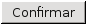
\includegraphics[scale=0.6]{12.Disenyo_Interfaz/12.3.Gestion_Informacion/12.3.4.Eliminacion_Elementos/botonConfirmar.png}
      \caption{Captura de pantalla del botón \textit{Confirmar}.}
      \label{capturaBotonConfirmar}
    \end{center}
  \end{figure}

